\begin{frame}[plain,noframenumbering]{Inhalt}
  \setbeamertemplate{section in toc}[sections numbered]
  \begin{columns}
  	\begin{column}{0.4\textwidth}
  		\Large
  		\tableofcontents
  	\end{column}
    \begin{column}{0.5\textwidth}
    	\begin{center}
    		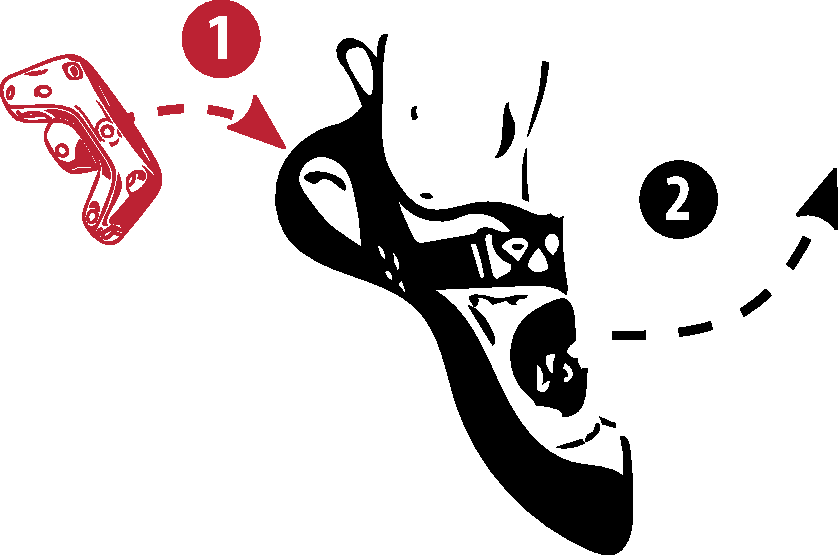
\includegraphics[width=0.8\columnwidth]{include/images/climbing-shoe-with-instructions-on.pdf}
    	\end{center}
  	\end{column}
  \end{columns}
\end{frame}

\section{Einleitung}

\begin{frame}{Motivation -- Zur Person}
  \begin{itemize}
    \item Kletter seit 20 Jahren
    \item Jugendleiter für Sportklettern
    \item mehrere eigene Forschungsprojekte
  \end{itemize}
\end{frame}

\begin{frame}{Eigene Forschungsprojekte -- Imagery in Sport Climbing}
\begin{figure}[h]
	\centering
	\begin{subfigure}[t]{0.49\columnwidth}
		\centering
		\begin{overpic}[width=\textwidth]{include/images/Google-Glass.jpg}
			\rbox{-1}{1}{\textcolor{source}{\tiny{Quelle: \href{https://de.wikipedia.org/wiki/Datei:Google_Glass_Main.jpg}{Wikipedia}}}}
		\end{overpic}
		\label{fig:google-glass}
	\end{subfigure}
	\hspace*{\fill}
	\begin{subfigure}[t]{0.49\columnwidth}
		\centering
		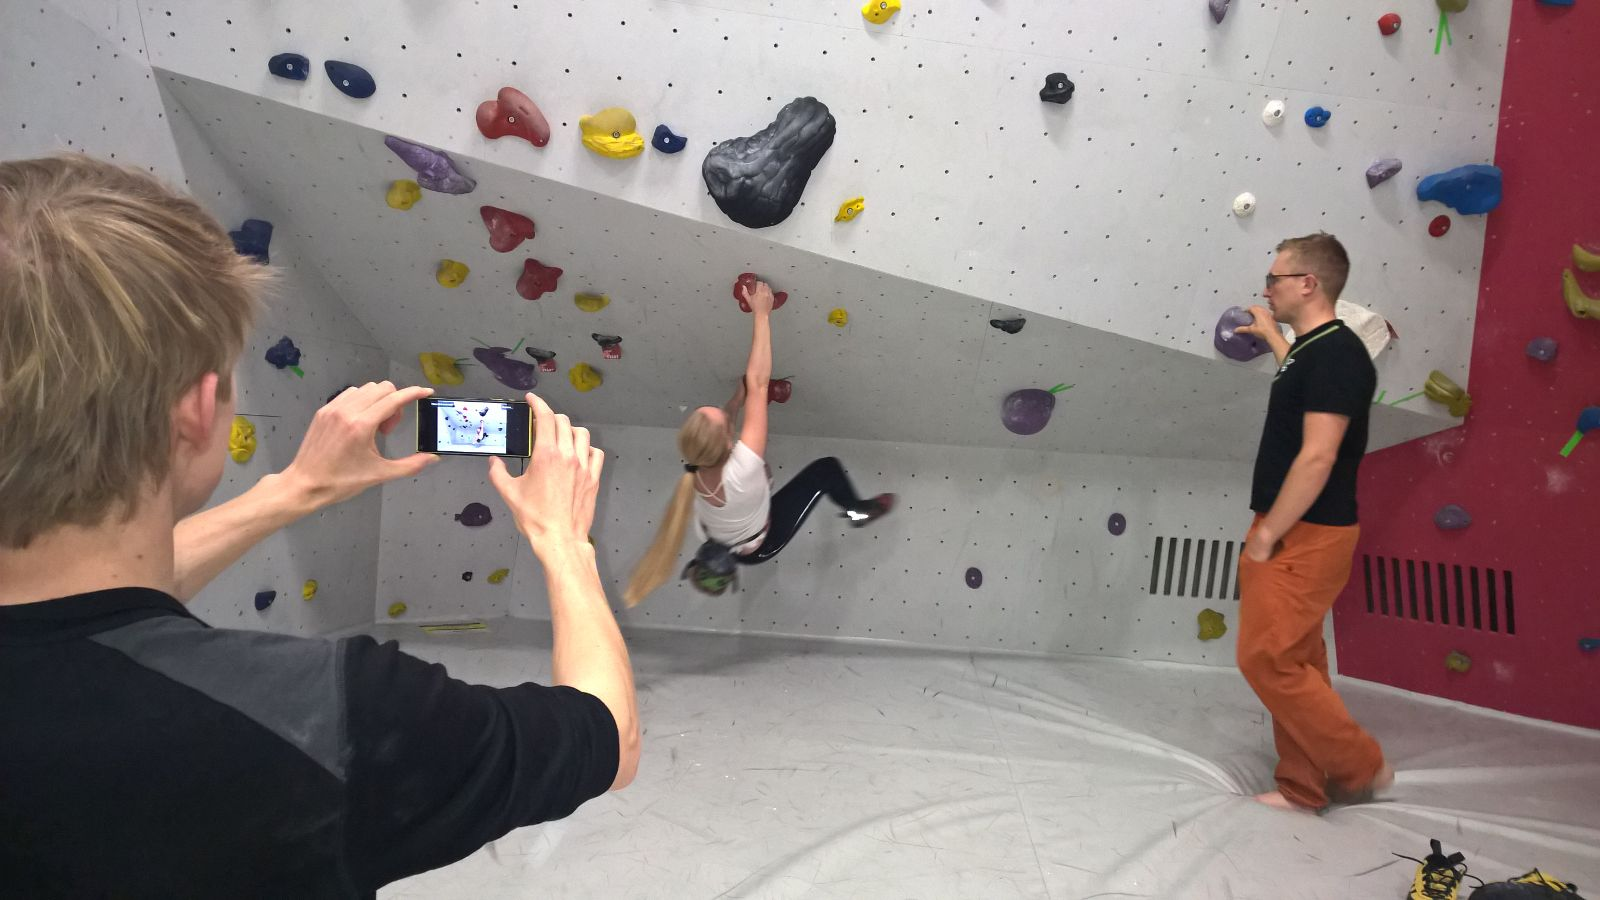
\includegraphics[width=\textwidth]{include/images/Live-Video.jpg}
		\label{fig:live-video-action}
	\end{subfigure}
	\caption{Livebildübertragung vom Smartphone (Kamera) an Google Glass Brille (Display). \\Die Kletterin kann sich selbst beim Klettern sehen, während sie klettert.}
	\label{fig:live-video}
\end{figure}
\end{frame}

\begin{frame}{Eigene Forschungsprojekte -- Crimp\textcolor{tracker}{Bit}}
\begin{figure}[h]
	\centering
	\begin{subfigure}[t]{0.35\columnwidth}
		\centering
		\begin{overpic}[width=\textwidth]{include/images/myo-armband.jpg}
			\rbox{-9}{1}{\textcolor{source}{\tiny{Quelle: \href{https://www.myo.com}{Thalmic Labs Inc.}}}}
		\end{overpic}
		\label{fig:myo-armband}
	\end{subfigure}
	\hspace*{\fill}
	\begin{subfigure}[t]{0.62\columnwidth}
		\centering
		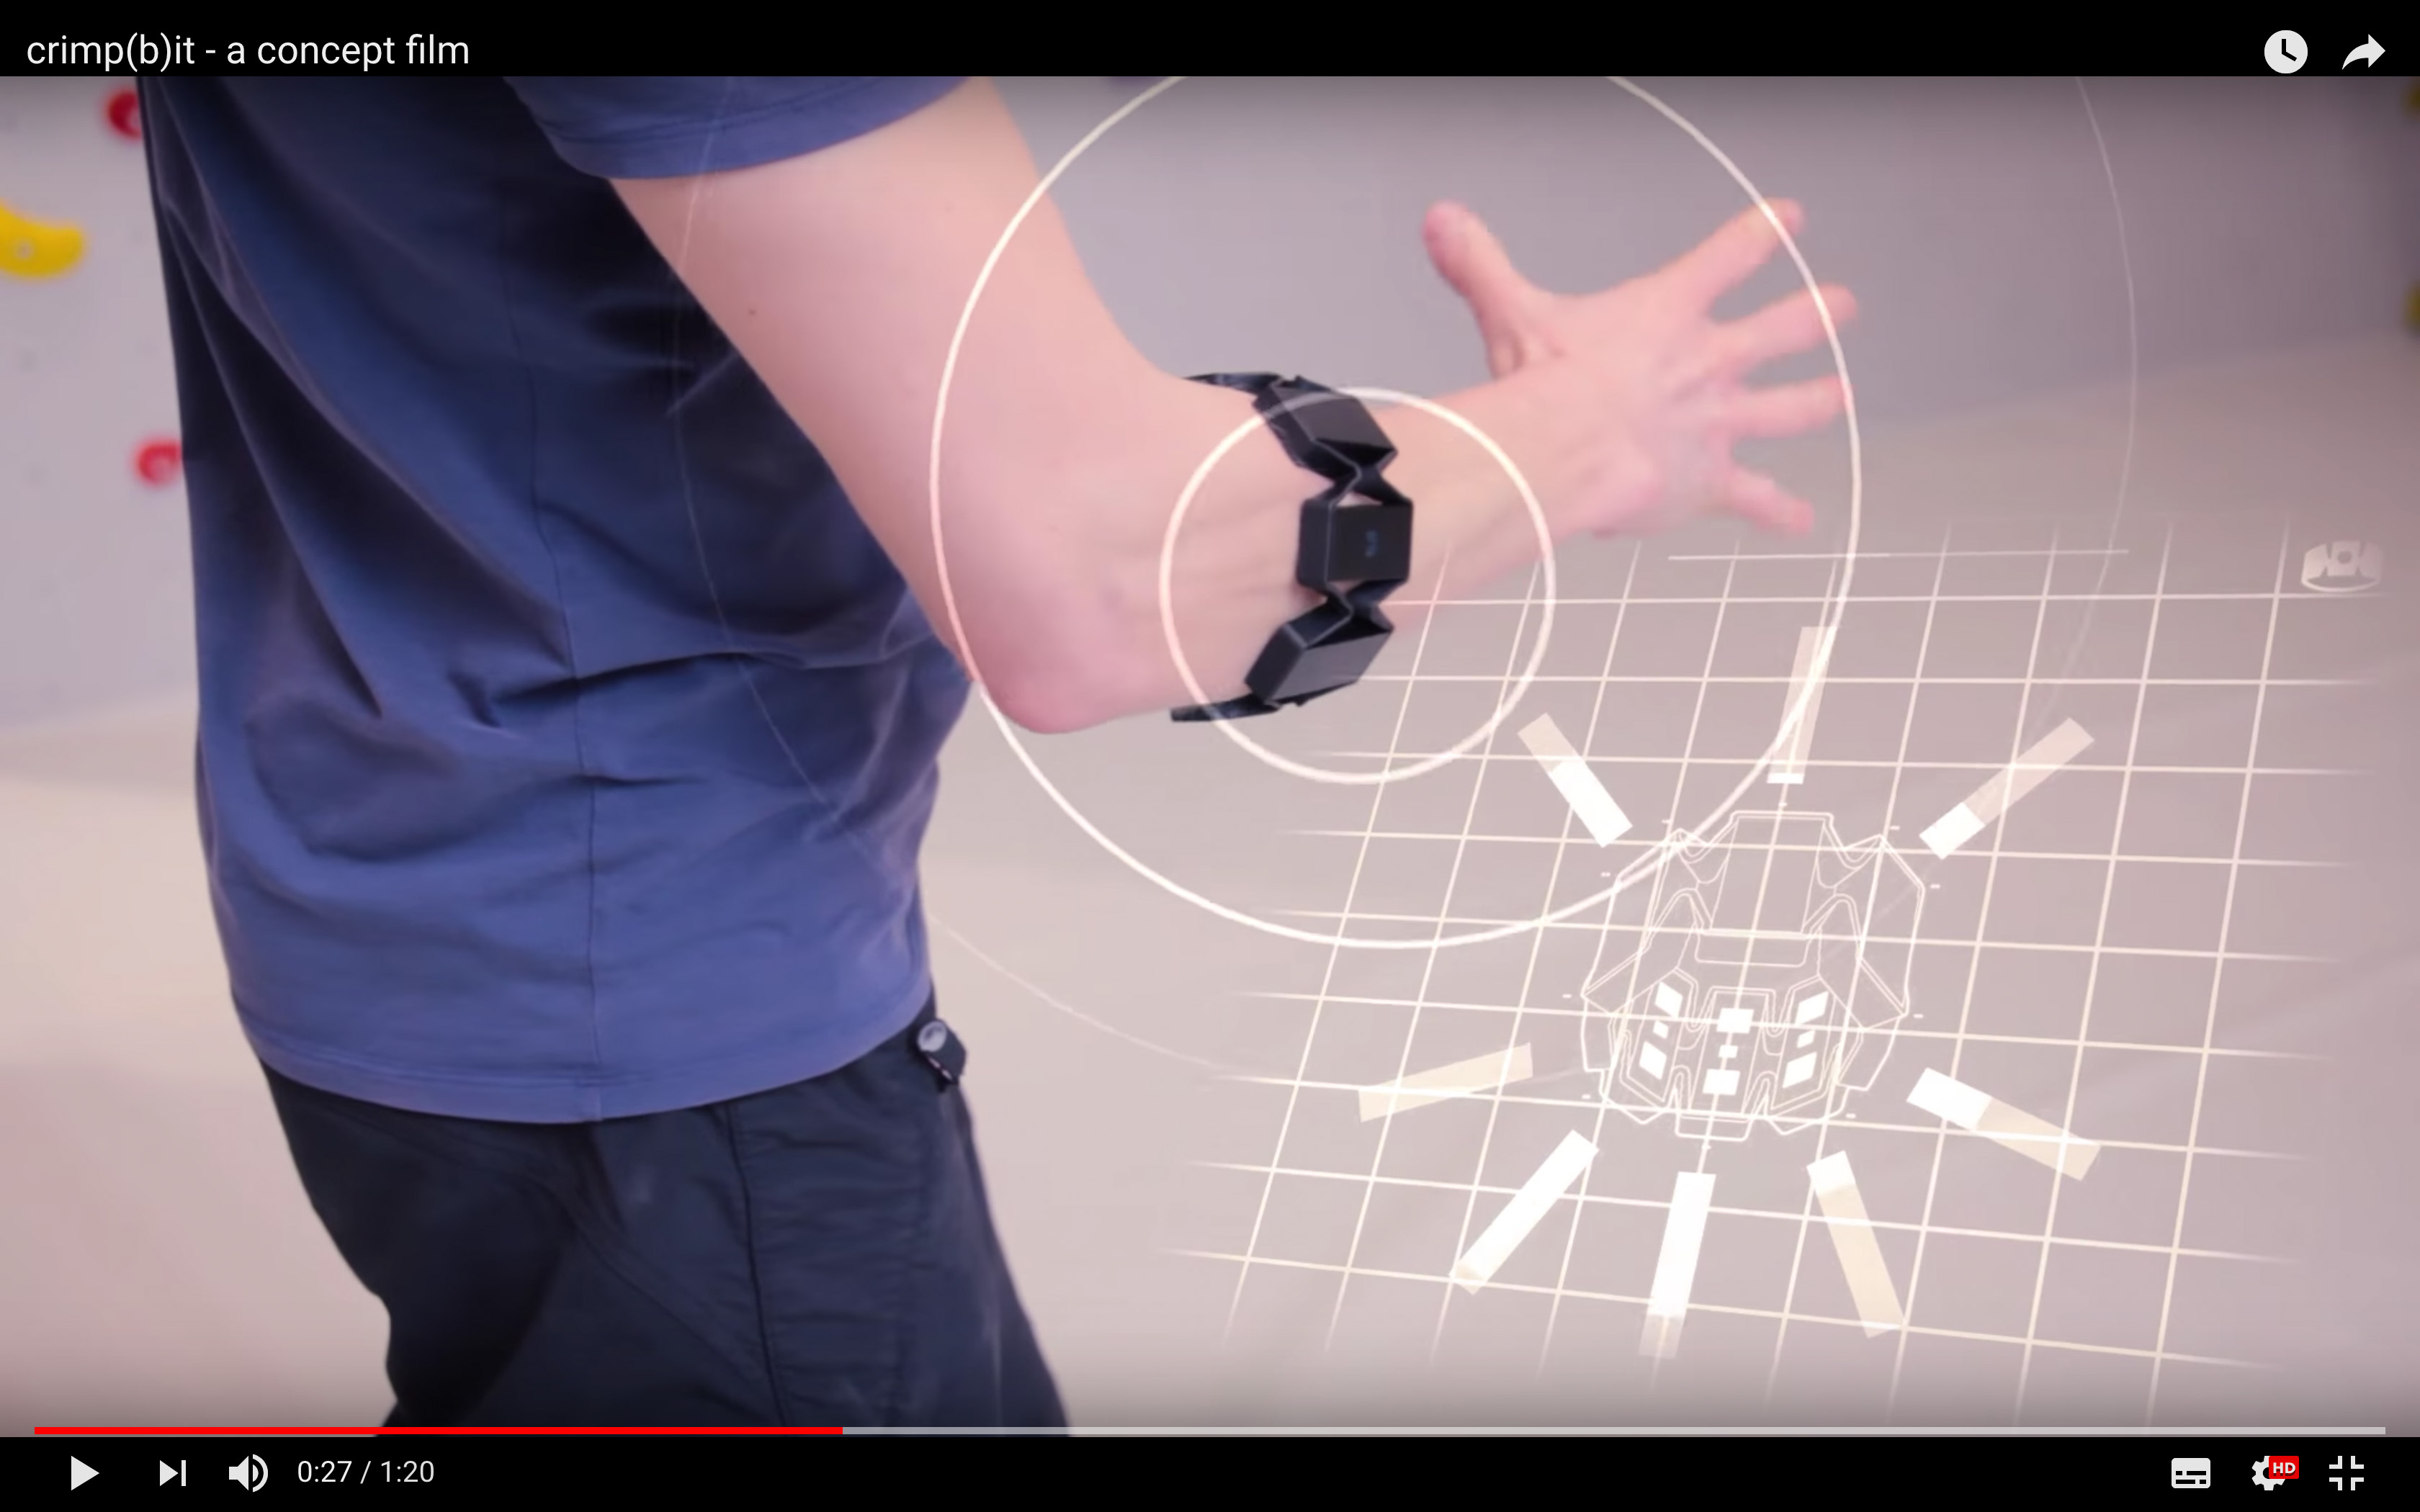
\includegraphics[width=\textwidth]{include/images/myo-demo.jpg}
		\label{fig:crimpbit-demo}
	\end{subfigure}
	\caption{MYO Armband zur Gestenerkennung als Sensor für potentiell schädliche Greifbewegungen.}
	\label{fig:crimpbit}
\end{figure}
\end{frame}

\begin{frame}{Motivation -- Grundlegende Fragestellung}
\begin{columns}
	\begin{column}{0.48\textwidth}
		\begin{itemize}
			\item zwei Professoren mit Kletterleidenschaft
			\item Forschungstrend \gls{VR}
			\item erfolgreicher Einsatz von \textit{\gls{VRET}} insbesondere \textit{bei Höhenangst} \autocite{Emmelkamp2001}
		\end{itemize}
	\end{column}
	\begin{column}{0.44\textwidth}
		\vfill
		\hfill
		\begin{overpic}[width=0.9\columnwidth]{include/images/samsung-gear-acrophobia-original.jpg}
			\rbox{-4}{1}{\textcolor{source}{\tiny{Quelle: \href{https://vrscout.com/projects/fear-of-heights-samsung-gear-vr/}{VRscout}}}}
		\end{overpic}
	\end{column}
\end{columns}
\vfill
\metroset{block=fill}
\begin{block}{Fragestellung}<2->
	Lässt sich \textcolor{tracker}{Sturzangst}, wie auch Höhenangst, \textcolor{tracker}{in \gls{VR} auslösen?}\\Wenn ja, welche Faktoren sind maßgebend?
	
	\hfill $\rightarrow$ Ist \gls{VR} als Trainingsmethoden denkbar?
\end{block}
\end{frame}

\begin{frame}{Verfeinerung der Fragestellung}
Was ist (Sturz-)Angst und wie lässt sie sich messen?\\Wie vergleiche ich Angst im Realen mit Angst im Virtuellen?
\begin{description}
\item[Immersion]<2-> Die technischen Möglichkeiten in ein virtuelle Welt einzutauchen,\\z.B. Bildschirm, grafische Darstellung, Ton \autocite{McMahan2003}
\item[Präsenz]<2-> Das aus Immersion resultierende Gefühl, vor Ort zu sein \autocite{McMahan2003}
\item[Angst]<3-> Mehrdimensionales Phänomen: Psych. u. Phys. Symptome \autocite{Krohne1996}
\item[Sturzangst]<3-> Angst vor dem Unkontrollierten, einer Verletzung \autocite{Lewis2010}
\end{description}
\begin{center}
	\only<4->{\large\textbf{Angeonommener Zusammenhang}\\Immersion $\sim$ Präsenz $\sim$ Angst }
\end{center}
\end{frame}

\begin{frame}{Forschungsfrage}
\begin{center}
	\LARGE
	$\substack{\text{Immersion}\\(\text{variieren})} \sim \substack{\text{Präsenz}\\(\text{messen})} \sim \substack{\text{Angst}\\(\text{messen})}$
\end{center}
\metroset{block=fill}
\begin{center}
	\begin{minipage}{0.7\textwidth}
		\begin{block}{Alternativ-Hypothese (H\textsubscript{a}\label{hyp:anxiety})}<2->
			Das \textcolor{tracker}{Präsenz}erleben von KletterInnen in \gls{VR} \textbf{steigt} wenn sie sich tatsächlich festhalten müssen, da dies die \textcolor{tracker}{Immersion} \textbf{erhöht} und damit die \textcolor{tracker}{Angst} \textbf{vergrößert}.
		\end{block}
		\begin{block}{Null-Hypothese (H\textsubscript{0}\label{hyp:anxiety})}<2->
			Es gibt keinen messbaren Unterschied zwischen Klettern in \gls{VR} mit \textcolor{tracker}{Griffen und Tritten} gegenüber Klettern in \gls{VR} mit \textcolor{tracker}{Game Controllern}.
		\end{block}
	\end{minipage}
\end{center}
\end{frame}

\begin{frame}{Studien zum Thema}
\begin{columns}
	\begin{column}{0.5\textwidth}
		Studien zur Auswirkung von (Sturz-)Höhe beim Sportklettern
		\autocites{Hardy2007}{Pijpers2006,Pijpers2005,Pijpers2003}
		\begin{center}
			\begin{overpic}[height=0.555\textheight]{include/images/pijpers.jpg}
				\rbox{-15}{1}{\textcolor{black}{\tiny{Quelle: \href{https://www.researchgate.net/figure/Side-view-of-the-virtual-environment-Subjects-start-in-the-Training-Room-and-later-enter_fig1_247181822}{ResearchGate}}}}
			\end{overpic}
		\end{center}
	\end{column}
	\begin{column}{0.5\textwidth}
		Studien Auswirkung unterschiedlicher Faktoren auf das Präsenzerleben
		\autocite{Meehan2002,Meehan2001}
		\begin{center}
			\begin{overpic}[height=0.6\textheight]{include/images/meehan.jpg}
				\rbox{-1}{1}{\textcolor{source}{\tiny{Quelle: \href{https://www.researchgate.net/figure/View-of-the-20-in-pit-from-the-wooden-ledge_fig3_7596875}{ResearchGate}}}}
			\end{overpic}
		\end{center}
		\vfill
	\end{column}
\end{columns}
\end{frame}

\section{Studie}

\begin{frame}{Versuchsbedingungen}
\begin{columns}
	\begin{column}{0.5\textwidth}
		\begin{enumerate}[label=\textbf\textcolor{tracker}{\Alph*}]
			\item Reales Klettern an Griffen und Tritten
			\\\textcolor{source}{\SI{10}{\meter} über Grund}
			\item Klettern in \gls{VR} an Griffen und Tritten
			\\\textcolor{source}{visuell \SI{10}{\meter} über Grund}
			\item Klettern in \gls{VR} mit Game Controllern
			\\\textcolor{source}{visuell \SI{10}{\meter} über Grund}
		\end{enumerate}
	\end{column}
	\begin{column}{0.5\textwidth}
		\begin{center}
			\vspace*{-15mm}
			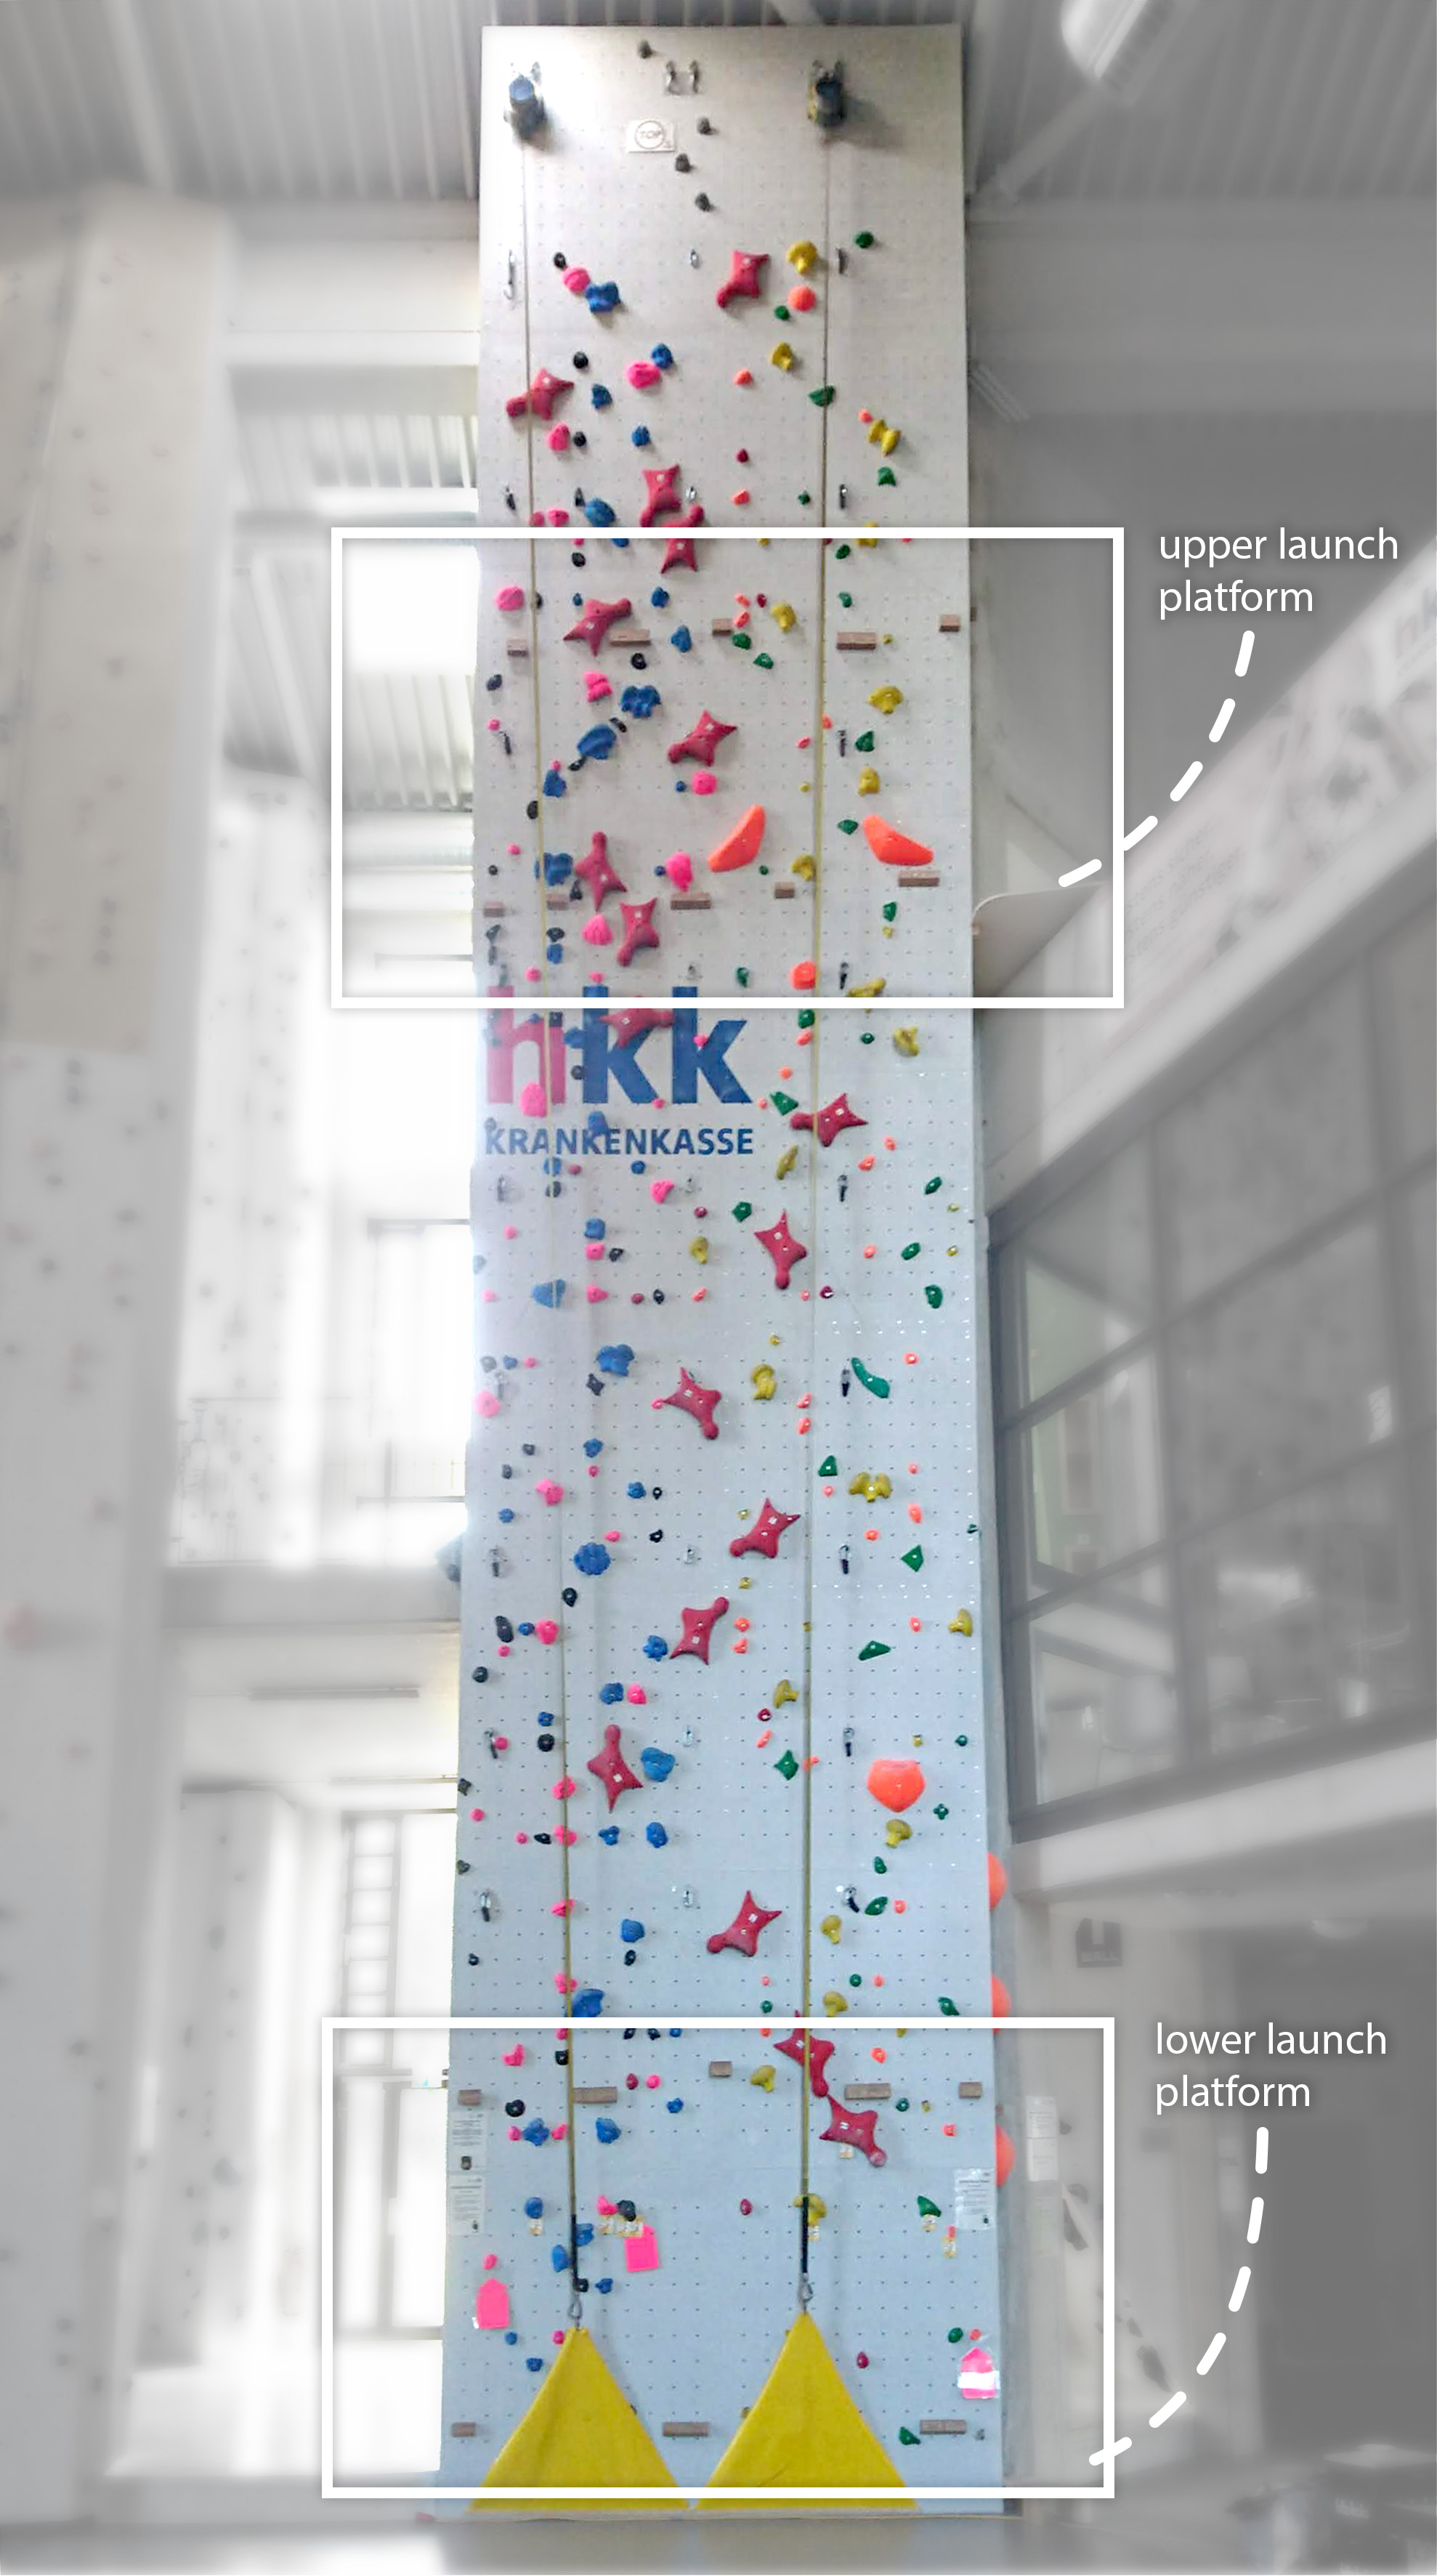
\includegraphics[height=1.2\textheight]{include/images/climbing-wall-photo.jpg}
		\end{center}
	\end{column}
\end{columns}
\end{frame}

\subsection{Technische Umsetzung}

\begin{frame}{Technische Umsetzung}

\end{frame}

\subsection{Methode}
\subsection{Ergebnisse}
\subsection{Diskussion}
\section{Fazit und Ausblick}

\begin{frame}[plain]
\begin{center}
	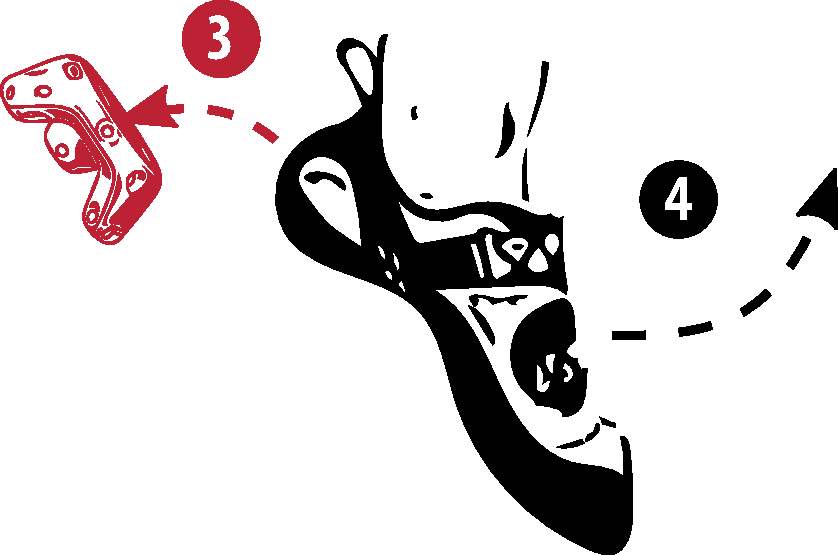
\includegraphics[width=0.8\textwidth]{include/images/climbing-shoe-with-instructions-off.pdf}
\end{center}
\end{frame}
